\chapter{静电场}
\section{电场力的性质}





1.电荷、电荷守恒定律和库仑定律

(1)元电荷、点电荷

\ding{172}元电荷:$e=1.60\times10^{-19}C$,所有带电体的电荷量都是元电荷的\_\_整数\_\_
倍;

\ding{173}点电荷:代表带电体的有一定电荷量的点,忽略带电体的大小和形状的理想化模型.

(2)电荷守恒定律

\ding{172}内容:电荷既不会创生,也不会消灭,它只能从一个物体转移到另一个物体,或者从物体的一部分转移到另一部分,在转移过程中,电荷的总量\_\_保持不变\_\_;

\ding{173}三种起电方式:\_\_摩擦\_\_起电、\_\_感应\_\_起电、\_\_接触\_\_起电;

\ding{174}带电实质:物体 \_\_得失电子\_\_;

\ding{175}电荷的分配原则:两个形状、大小相同且带同种电荷的导体,接触后再分开,二者带\_\_相同\_\_电荷,若两导体原来带异种电荷,则电荷先\_\_中和\_\_,余下的电荷再\_\_平分\_\_.

(3)库仑定律

\ding{172}内容;\_\_真空\_\_中两个静止\_\_点电荷\_\_之间的相互作用力,与它们的电荷量的乘积成\_\_正比\_\_,与它们的距离的二次方成\_\_反比\_\_,作用力的方向在它们的连线上;

\ding{173}表达式:$F=k\dfrac{q_1q_2}{r^2}$,式中k=\_\_$9.0\times 10^9$\_\_$N\cdot m^2/C^2$,叫做静电力常量;

\ding{174}适用条件:\_\_真空\_\_中的\_\_点电荷\_\_.

a.在空气中,两个点电荷的作用力近似等于真空中的情况,可以直接应用公式,

b.当两个带电体的间距远大于本身的大小时,可以把带电体看成点电荷.

\ding{175}库仑力的方向:由相互作用的两个带电体决定,即同种电荷相互\_\_排斥\_\_,异种电荷相互\_\_吸引\_\_.

2.电场、电场强度

(1)电场

\ding{172}定义:存在于电荷周围,能传递电荷间相互作用的一种特殊物质;

\ding{173}基本性质;对放入其中的电荷有\_\_力的作用\_\_.

(2)电场强度

\ding{172}定义:放入电场中某点的电荷受到的电场力F与它的电荷量q的比值;

\ding{173}定义式:$E=\dfrac{F}{q}$;单位:N/C或\_\_V/m\_\_;

\ding{174}矢量性:规定\_\_正电荷\_\_在电场中某点所受电场力的方向为该点电场强度的方向.

3.电场线

(1)定义

为了形象地描述电场中各点场强的强弱及\_\_方向\_\_,在电场中画出一些曲线,曲线上每一点的\_\_切线\_\_方向都跟该点的场强方向一致,曲线的疏密表示电场的\_\_强弱\_\_.

(2)电场线的特点

\ding{172}电场线从\_\_正电荷\_\_或\_\_无限远\_\_处出发,终止于\_\_负电荷\_\_或\_\_无限远\_\_处;

\ding{173}电场线在电场中不相交,也不相切;

\ding{174}在同一幅图中,电场强度较大的地方电场线\_\_较密集\_\_,电场强度较小的地方电场线\_\_较稀疏\_\_.

\newpage


\subsection{三个自由点电荷的平衡问题}

{[}例1{]}如图所示,$q_1$、$q_2$、$q_3$分别表示在一条直线上的三个点电荷,已知$q_1$与$q_2$之间的距离为$l_1$,$q_2$与$q_3$之间的距离为$l_2$,且三个点电荷都处于平衡状态.

\begin{center}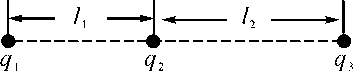
\includegraphics[width=1.60417in,height=0.32292in]{media/image260.png}\end{center}

(1)若$q_2$为负电荷,则$q_1$为\_\_正电\_\_电荷,$q_3$为\_\_正电\_\_电荷;

(2)$q_1$、$q_2$、$q_3$的电荷量大小之比是\_\_2:1:2\_\_.

解析 (1)假设$q_1$、$q_3$均带负电,则虽然$q_2$可以平衡,但$q_1$(或$q_3$)所受的两个库仑力均为斥力,故而方向相同,不能平衡.假设$q_1$、$q_3$均带正电,则每个点电荷所受的两个库仑力均方向相反,可能平衡.因此,$q_1$、$q_3$均带正电.也就是说,在这种情况下,$q_1$、$q_3$必须是同种电荷且跟$q_2$是异种电荷.

(2)$q_1$受$q_2$水平向右的库仑引力作用和$q_3$水平向左的库仑斥力作用.

由库仑定律和力的平衡条件有$k\dfrac{q_1q_2}{l_1^2}=k\dfrac{q_1q_3}{(l_1+l_2)^2}$,

同理,对$q_2$有$k\dfrac{q_1q_2}{l_1^2}=k\dfrac{q_2q_3}{l_2^2}$,

对$q_3$有$k\dfrac{q_2q_3}{l_2^2}=k\dfrac{q_1q_3}{(l_1+l_2)^2}$,

由以上三式得$q_1$:$q_2$:$q_3$=$(\dfrac{l_1+l_2}{l_2} )^2:1:(\dfrac{l_1+l_2}{l_1} )^2$.

\begin{center}
\includegraphics[width=0.70833in,height=0.125in]{media/image13.png}

\textbf{三个自由点电荷的平衡问题}
\end{center}


(1)条件

两个点电荷在第三个点电荷处的合电场强度为零,或每个点电荷受到的两个库仑力必须大小相等,方向相反.

(2)规律

\ding{172}``三点共线''------三个点电荷分布在同一条直线上;

\ding{173}``两同夹异''------正负电荷相互间隔;

\ding{174}``两大夹小''------中间电荷的电荷量最小;

\ding{175}``近小远大''------中间电荷靠近电荷量较小的电荷.
\newpage
\subsection{库仑力作用下的共点力平衡问题}

\begin{center}
\includegraphics[width=0.70833in,height=0.125in]{media/image37.png}

\textbf{解决库仑力作用下平衡问题的方法}
\end{center}


库仑力作用下平衡问题的分析方法与纯力学平衡问题的分析方法是相同的,只是在原来受力的基础上多了电场力.

{[}例2{]}(多选)如图所示,水平地面上固定一个光滑绝缘斜面,斜面与水平面的夹角为$\theta$.一根轻质绝缘细线的一端固定在斜面顶端,另一端系有一个带电小球A,细线与斜面平行,小球A的质量为m、电荷量为q.小球A的右侧固定放置带等量同种电荷的小球B,两球心的高度相同、间距为d.静电力常量为k,重力加速度为g,两带电小球可视为点电荷.小球A静止在斜面上,则( AC )

\begin{center}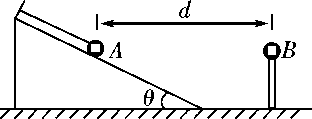
\includegraphics[width=1.41667in,height=0.54167in]{media/image261.png}\end{center}

A.小球A与B之间库仑力的大小为$\dfrac{kq^2}{d^2}$

B.当$\dfrac{q}{d}=\sqrt{\dfrac{mg\sin\theta}{k}}$时,细线上的拉力为0

C.当$\dfrac{q}{d}=\sqrt{\dfrac{mg\tan\theta}{k}}$时,细线上的拉力为0

D.当$\dfrac{q}{d}=\sqrt{\dfrac{mg}{k\tan\theta}}$时,斜面对小球A的支持力为0

解析 根据库仑定律可得两小球之间的库仑力大小为$F=\dfrac{kq^2}{d^2}$,选项A正确;当细线上的拉力为零时,小球A受到库仑力、斜面支持力、重力,由平衡条件得$\dfrac{kq^2}{d^2}=mg\tan\theta$,解得$\dfrac{q}{d}=\sqrt{\dfrac{mg\tan\theta}{k}}$,选项B错误,C正确;由受力分析可知,斜面对小球的支持力不可能为零,选项D错误.

\begin{center}
\includegraphics[width=0.70833in,height=0.125in]{media/image25.png}\end{center}
\begin{center}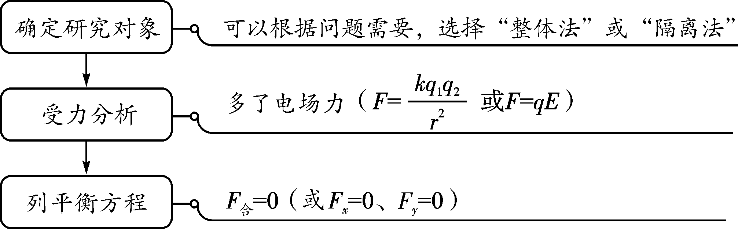
\includegraphics[width=3.35417in,height=1.04167in]{media/image262.png}\end{center}
\newpage
\subsection{电场强度的理解和应用}

1.电场强度三个表达式的比较

\begin{longtable}[]{@{}m{2cm}m{4cm}m{4cm}m{3cm}@{}}
\toprule

表达式比较&$E=\dfrac{F}{q}$&$E=k\dfrac{Q}{r^2}$&$E=\dfrac{U}{d}$
\tabularnewline
\midrule
\endhead
公式意义 & 电场强度定义式 & 真空中点电荷的电场强度决定式 &
匀强电场中E与U的关系式\tabularnewline
适用条件 & 一切电场 & 真空中点电荷的电场 & 匀强电场\tabularnewline
决定因素 & 由电场本身决定,与检验电荷q无关,q充当测量工具 &
由场源电荷Q和场源电荷到该点的距离r共同决定 &
由电场本身决定,d为两点沿电场方向的距离\tabularnewline
\bottomrule
\end{longtable}

2.电场的叠加

(1)叠加原理:多个电荷在空间某处产生的电场为各电荷在该处所产生的电场强度的矢量和.

(2)运算法则:平行四边形定则.

{[}例3{]}如图所示,直角坐标系xOy中,M、N两点位于x轴上,G、H两点坐标如图所示.M、N两点各固定一负点电荷,一电荷量为Q的正点电荷置于O点时,G点处的电场强度恰好为零.静电力常量用k表示.若将该正点电荷移到G点,则H点处场强的大小和方向分别为( B )

\begin{center}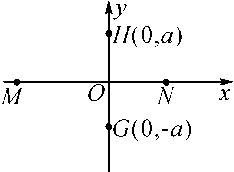
\includegraphics[width=1.0625in,height=0.78125in]{media/image263.png}\end{center}

A.$\dfrac{3kQ}{4a^2}$沿y轴正向   B.$\dfrac{3kQ}{4a^2}$沿y轴负向

C.$\dfrac{5kQ}{4a^2}$沿y轴正向   D.$\dfrac{5kQ}{4a^2}$沿y轴负向

\begin{center}
\includegraphics[width=0.70833in,height=0.125in]{media/image13.png}

\textbf{分析电场叠加问题的一般步骤}
\end{center}


电场强度是矢量,叠加时应遵从平行四边形定则.

分析电场的叠加问题的一般步骤:

(1)确定分析计算的空间位置;

(2)分析该处有几个分电场,先计算出各个分电场在该点的电场强度的大小和方向;

(3)依次利用平行四边形定则求出矢量和.
\newpage
\subsection{电场线的理解和应用}

1.电场线的对称性

\begin{center}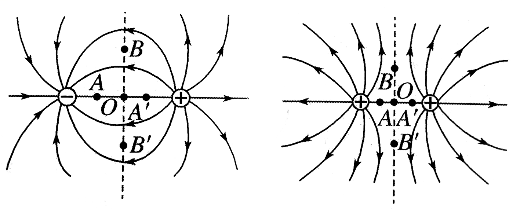
\includegraphics[width=2.36458in,height=0.94792in]{media/image264.png}\end{center}

(1)两等量同种点电荷连线及中垂线上关于O点对称的点的电场强度等大反向.

(2)两等量异种点电荷连线及中垂线上关O点对称的点的电场强度等大同向.

2.电场线的应用

\begin{center}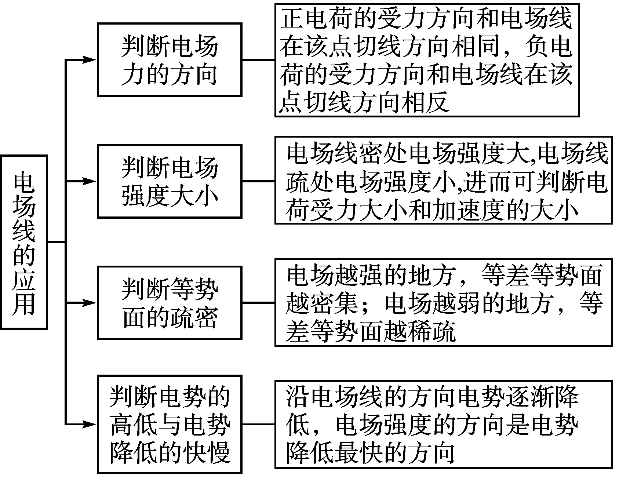
\includegraphics[width=2.8125in,height=2.16667in]{media/image265.png}\end{center}
{[}例4{]}如图所示,实线为不知方向的三条电场线,从电场中M点以相同速度垂直于电场线方向飞出a、b两个带电粒子,运动轨迹如图中虚线所示.则( C )

\begin{center}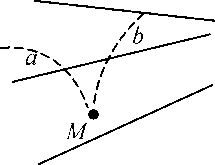
\includegraphics[width=0.97917in,height=0.75in]{media/image266.png}\end{center}

A.a一定带正电,b一定带负电

B.a的速度将减小,b的速度将增加

C.a的加速度将减小,b的加速度将增加

D.两个粒子的动能,一个增加一个减小

\begin{center}
\includegraphics[width=0.70833in,height=0.125in]{media/image13.png}\end{center}

(1)由粒子运动轨迹判断粒子运动情况

(2)由粒子受力方向指向曲线的内侧,且与电场线相切.从而判断电场的方向.

(3)由电场线的疏密判断加速度大小.

(4)由电场力做功的正负判断粒子动能的变化情况.

\subsection{对称法在电场叠加中的应用}

对称现象普遍存在于各种物理现象和物理规律中,应用对称性不仅能帮助我们认识和探索某些基本规律,而且也能帮助我们去求解某些具体的物理问题.利用对称法分析解决物理问题,可以避免复杂的数学演算和推导,直接抓住问题的特点,出奇制胜,快速简便地求解问题.

\begin{center}
\includegraphics[width=0.70833in,height=0.125in]{media/image37.png}

\textbf{对称法在电场叠加中的应用技巧}
\end{center}


(1)有些物理题不具有对称性,直接求解比较困难,但采取割补法却使问题迎刃而解.

(2)该法的核心思想就是变不对称为对称.

{[}例5{]}(2017·湖北黄冈诊断)均匀带电的球壳在球外空间产生的电场等效于电荷集中于球心处产生的电场.如图所示,在半球面AB上均匀分布正电荷,总电荷量为q,球面半径为R,CD为通过半球面顶点与球心O的轴线,在轴线上有M、N两点,OM=ON=2R.已知M点的场强大小为E,则N点的场强大小为( A )

\begin{center}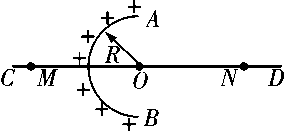
\includegraphics[width=1.29167in,height=0.59375in]{media/image267.png}\end{center}

A.$\dfrac{kq}{2R^2}-E$ 

B.$\dfrac{kq}{4R^2}$

C.$\dfrac{kq}{4R^2}-E$ 

D.$\dfrac{kq}{4R^2}+E$

解析 左半球面AB上的正电荷产生的电场等效为带正电荷为2q的整个球面的电场和带电荷-q的右半球面的电场的合电场,则$E=\dfrac{2kq}{(2R)^2}-E'$,$E'$为带电荷-q的右半球面在M点产生场强大小.带电荷-q的右半球面在M点的场强大小与带正电荷为q的左半球面AB在N点的场强大小相等,则$E_N=E'=\dfrac{2kq}{(2R)^2} -E=\dfrac{kq}{2R^2} -E$,则选项A正确.
\newpage
\section{电场能的性质}


1.电势能和电势 等势面

(1)静电力做功

\ding{172}特点:静电力做功与路径无关,只与\_\_初末位置\_\_有关.

\ding{173}计算方法

a.$W=qEd$,只适用于\_\_匀强\_\_电场,其中d为沿\_\_电场方向\_\_的距离.

b.$W_{A B}=q U_{A B}$,适用于\_\_任何\_\_电场.

(2)电势能

\ding{172}定义:电荷在电场中某点具有的势能,等于将电荷从该点移到\_\_零势点\_\_位置时电场力所做的功.

\ding{173}电场力做功与电势能变化的关系:电场力做的功等于\_\_电势能增量的负值\_\_,即$W_{A B}=E_{\mathrm{pA}}-E_{\mathrm{p} B}=-\Delta E_{\mathrm{p}}$.

(3)电势

\ding{172}定义:电荷在电场中某点具有的\_\_电势能\_\_与它的\_\_电荷量\_\_的比值.

\ding{173}定义式:$\varphi=\dfrac{E_{p}}{q}$.

\ding{174}矢标性:电势是标量,有正负之分,其正(负)表示该点电势比零势点高(低).

\ding{175}相对性,电势具有\_\_相对性\_\_,同一点的电势因选取\_\_零势点\_\_的不同而不同,通常取无限远或地球的电势为零.

(4)等势面的特点

\ding{172}同一等势面上的任意两点间移动电荷电场力\_\_不做功\_\_.

\ding{173}等势面一定跟电场线\_\_垂直\_\_,即跟场强的方向\_\_垂直\_\_.

\ding{174}电场线总是从电势较\_\_高\_\_的等势面指向电势较\_\_低\_\_的等势面.

\ding{175}等差等势面越密的地方场强越大,反之越\_\_小\_\_.

2.电势差 匀强电场中电势差与场强的关系

(1)电势差

\ding{172}定义:电荷在电场中,由一点A移到另一点B时,\_\_电场力F做的功\_\_与移动的电荷的\_\_电荷量\_\_的比值.

\ding{173}定义式:$U_{A B}=\dfrac{W_{A B}}{q}$.

\ding{174}电势差与电势的关系,$U_{A B}=\varphi_{A}-\varphi_{B}, U_{A B}=-U_{B A}$.

\ding{175}影响因素:电势差$U_{A B}$由电场本身的性质决定,与移动的电荷q及电场力做的功$W_{AB}$\_\_无关\_\_,与零电势点的选取\_\_无关\_\_.

(2)匀强电场中电势差与电场强度的关系

\ding{172}电势差与电场强度的关系式,$U_{A B}=E d$,其中d为A、B两点\_\_沿电场方向\_\_的距离.

\ding{173}在匀强电场中,电场强度在数值上等于沿\_\_电场强度\_\_方向每单位距离上降低的电势;

注意:电场中,沿电场强度方向电势降落得最快.


\newpage


\subsection{电势高低与电势能大小的判断}

1.电势高低的判断

\begin{longtable}[]{@{}m{3.5cm}m{11cm}@{}}
\toprule
判断角度 & 判断方法\tabularnewline
\midrule
\endhead
依据电场线方向 & 沿电场线方向电势逐渐降低\tabularnewline
依据场源电荷的正负 &
取无穷远处电势为零,正电荷周围电势为正值,负电荷周围电势为负值,靠近正电荷处电势高,靠近负电荷处电势低\tabularnewline
依据电场力做功 &
根据$U_{A B}=\dfrac{W_{A B}}{q}$,将$W_{A B}$、$q$的正负号代入,由$U_{A B}$的正负判断$\varphi _A$、$\varphi_B$的高低\tabularnewline
依据电势能的高低 &
正电荷在电势较高处电势能大,负电荷在电势较低处电势能大\tabularnewline
\bottomrule
\end{longtable}

2.电势能大小的判断

\begin{longtable}[]{@{}m{2cm}m{13cm}@{}}
\toprule
判断角度 & 判断方法\tabularnewline
\midrule
\endhead
做功判断法&电场力做正功,电势能减小;电场力做负功,电势能增加\tabularnewline
电荷电势法&正电荷在电势高的地方电势能大;负电荷在电势低的地方电势能大\tabularnewline
公式法 &
将电荷量、电势连同正负号一起代入公式正$E_{\mathrm{p}}=q \varphi$,正$E_p$的绝对值越大,电势能越大;负$E_p$的绝对值越大,电势能越小\tabularnewline
能量守恒法 &
在电场中,若只有电场力做功时,电荷的动能和电势能相互转化,动能增加,电势能减小,反这,动能减小,电势能增加\tabularnewline
\bottomrule
\end{longtable}

\begin{center}
\includegraphics[width=0.70833in,height=0.125in]{media/image37.png}

\textbf{静电场中几个物理概念之间的关系}
\end{center}


(1)电场线与电场强度的关系:电场线越密的地方表示电场强度越大,电场线上某点的切线方向表示该点的电场强度方向.

(2)电场线与等势面的关系:电场线与等势面垂直,并从电势较高的等势面指向电势较低的等势面.

(3)电势能与电势的关系:正电荷在电势高的地方电势能大;负电荷在电势低的地方电势能大.



\begin{center}
\includegraphics[width=0.70833in,height=0.125in]{media/image13.png}\end{center}
电场中各点的电势与试探电荷无关;电荷在电场中某点的电势能与试探电荷有关;在电场中移动电荷,电场力做功和电势能的变化都与电荷有关.
\newpage
\subsection{等势面与粒子运动轨迹的分析}

1.几种常见的典型电场的等势面比较

\begin{longtable}[]{@{}m{3cm}m{4cm}m{5cm}@{}}
\toprule
电场 & 等势面(实线)图样 & 重要描述\tabularnewline
\midrule
\endhead
匀强电场 & 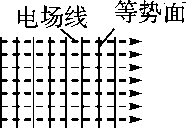
\includegraphics[width=0.84375in,height=0.58333in]{media/image276.png} &垂直于电场线的一簇平面\tabularnewline
点电荷的电场 &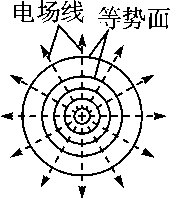
\includegraphics[width=0.77083in,height=0.90625in]{media/image277.png} &以点电荷为球心的一簇球面\tabularnewline

等量异种点电荷的电场& 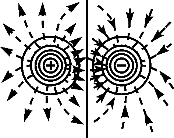
\includegraphics[width=0.79167in,height=0.625in]{media/image278.png}& 连线的中垂线上的电势为零\tabularnewline

等量同种正点电荷的电场& 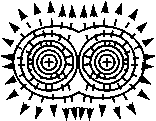
\includegraphics[width=0.70833in,height=0.55208in]{media/image279.png}& 连线上,中点电势最低,而在中垂线上,中点电势最高\tabularnewline
\bottomrule
\end{longtable}

2.带电粒子在电场中运动轨迹问题的分析方法

(1)从轨迹的弯曲方向判断受力方向(轨迹向合外力方向弯曲),从而分析电场方向或电荷的正负;

(2)结合轨迹、速度方向与静电力的方向,确定静电力做功的正负,从而确定电势能、电势和电势差的变化等;

(3)根据动能定理或能量守恒定律判断动能的变化情况.

\begin{center}
\includegraphics[width=0.70833in,height=0.125in]{media/image25.png}

\textbf{带电粒子在电场中运动轨迹的分析思路}
\end{center}


\begin{center}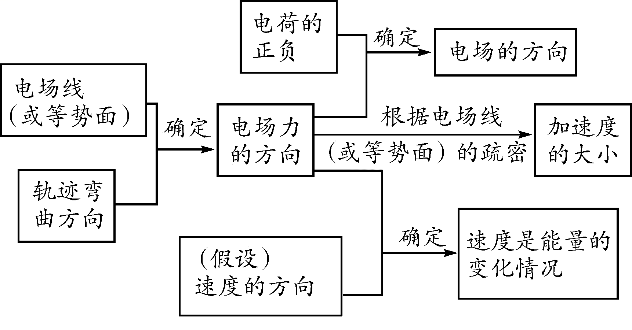
\includegraphics[width=2.875in,height=1.5in]{media/image280.png}\end{center}

\newpage
\subsection{电势差与电场强度的关系}

1.匀强电场中电势差与电场强度的关系

(1)$U_{A B}=E d$,d为A、B两点沿电场方向的距离.

(2)沿电场强度方向电势降落得最快.

2.$E=\dfrac{U}{d}$在非匀强电场中的几点妙用

(1)解释等差等势面的疏密与电场强度大小的关系,当电势差U一定时,电场强度E越大,则沿电场强度方向的距离d越小,即电场强度越大,等差等势面越密.

(2)定性判断非匀强电场电势差的大小关系,如距离相等的两点间的电势差,E越大,U越大;E越小,U越小.

\begin{center}
\includegraphics[width=0.70833in,height=0.125in]{media/image37.png}

\textbf{匀强电场中的两点推论}
\end{center}


(1)如图甲,C点为线段AB的中点,则有$\varphi_{C}=\dfrac{\varphi_{A}+\varphi_{B}}{2}$.

(2)如图乙,$A B \| C D$,且AB=CD,则$U_{A B}=U_{C D}$.

\begin{center}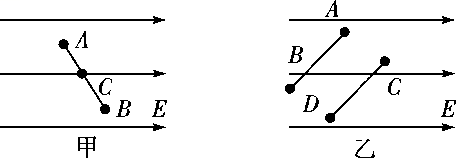
\includegraphics[width=2.07292in,height=0.71875in]{media/image282.png}\end{center}
{[}例3{]}(2017·全国卷\uppercase\expandafter{\romannumeral3})(多选)一匀强电场的方向平行于xOy平面,平面内a、b、c三点的位置如图所示,三点的电势分别为10
V、17 V、26 V.下列说法正确的是( ABD )

\begin{center}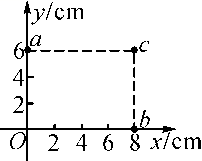
\includegraphics[width=0.91667in,height=0.72917in]{media/image283.png}\end{center}

A.电场强度的大小为2.5 V/cm

B.坐标原点处的电势为1 V

C.电子在a点的电势能比在b点的低7 eV

D.电子从b点运动到c点,电场力做功为9 eV

解析 ac垂直于bc,沿ca和cb两方向的场强分量大小分别为$E_{x}=\dfrac{U_{c a}}{a c}=2 \mathrm{V} / \mathrm{cm}, E_{y}=\dfrac{U_{c b}}{b c}=1.5 \mathrm{V} / \mathrm{cm}$,根据矢量合成可知E=2.5V/cm.选项A正确;根据在匀强电场中平行线上等距同向的两点间电势差相等,有$\varphi_{0}-\varphi_{a}=\varphi_{b}-\varphi_{c}$,得$\varphi_{0}=1V$,选项B正确;由于在a、b、c三点的电势能分别为-10 eV,-17 eV和-26eV,故电子在a点的电势能比在b点的高7eV,选项C错误;电子从b点运动到c点,电场力做功W=(-17 eV)-(-26 eV)=9eV,选项D正确.

\subsection{图象在电场中的应用}

1.v-t图象

根据v-t图象的速度变化、斜率变化(即加速度大小的变化),确定电荷所受电场力的方向与电场力的大小变化情况,进而确定电场强度的方向、电势的高低及电势能的变化.

{[}例4{]}(2018·四川宜宾模拟)(多选)如图甲所示,直线MN表示某电场中一条电场线,a、b是线上的两点,将一带负电荷的粒子从a点处由静止释放后,粒子仅在电场力的作用下从a运动到b过程中的v-t图线如图乙所示.设a、b两点的电势分别为$\varphi_a$、$\varphi_b$,电场强度的大小分别为$E_a$、$E_b$,粒子在a、b两点的电势能分别为$W_a$、$W_b$,不计重力,则有( BD )

\begin{center}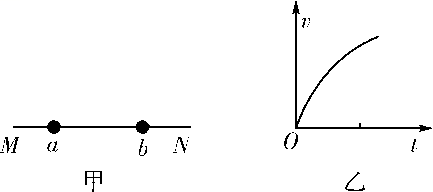
\includegraphics[width=1.96875in,height=0.875in]{media/image284.png}\end{center}

A.$\varphi_a$\textgreater $\varphi_b$   

B.$E_a$\textgreater $E_b$

C.$E_a$\textless $E_b$   

D.$W_a$\textgreater $W_b$

2.$\varphi -x$图象

(1)电场强度的大小等于$\varphi -x$图线的斜率大小,电场强度为零处,$\varphi -x$图线存在极值,其切线的斜率为零.

(2)在$\varphi -x$图象中可以直接判断各点电势的大小,并可根据电势大小关系确定电场强度的方向.

(3)在$\varphi -x$图象中分析电荷移动时电势能的变化,可用$W_{AB}$=$qU_{AB}$,进而分析$W_{AB}$的正负,然后作出判断.

{[}例5{]}(2018·重庆模拟)两电荷量分别为$q_1$和$q_2$的点电荷放在x轴上的O、M两点,两电荷连钱上各点电势$\varphi$随x变化的关系如图所示,其中A、N两点的电势均为零,ND段中的C点电势最高,则( D )

\begin{center}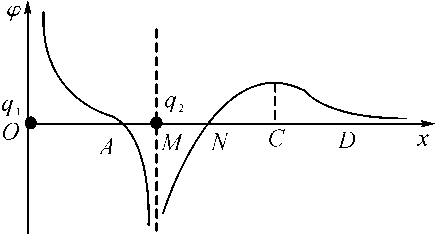
\includegraphics[width=1.97917in,height=1.0625in]{media/image285.png}\end{center}

A.N点的电场强度大小为零

B.A点的电场强度大小为零

C.NC间电场强度方向指向x轴正方向

D.将一负点电荷从N点移到D点,电场力先做正功后做负功
\newpage
3.E-x图象

(1)反映了电场强度随位移变化的规律.

(2)E\textgreater0表示场强沿x轴正方向;E\textless0表示场强沿x轴负方向.

(3)图线与x轴围成的``面积''表示电势差,``面积''大小表示电势差大小,两点的电势高低根据电场方向判定.

{[}例6{]}(2018·河南开封模拟)(多选)空间存在一静电场,其在x轴上的电场强度E随x的变化关系如图所示,x轴正方向为场强正方向,带正电的点电荷沿x轴水平向右运动,则点电荷( BC )

\begin{center}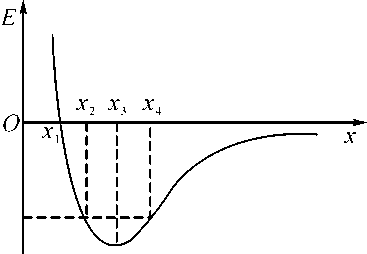
\includegraphics[width=1.66667in,height=1.15625in]{media/image286.png}\end{center}

A.在$x_2$和$x_4$处电势能相等

B.由$x_1$运动到$x_3$的过程中电势能增大

C.从$x_1$运动到$x_4$的过程中电场力先增大后减小

D.从$x_1$运动到$x_4$的过程中电场力先减小后增大

\newpage
\section{电容器 带电粒子在电场中的运动}





1.电容器及电容

(1)电容器

\ding{172}组成:由两个彼此\_\_绝缘\_\_又相互靠近的导体组成;

\ding{173}带电荷量:一个极板所带电荷量的\_\_绝对值\_\_;

\ding{174}电容器的充、放电

a.充电:使电容器带电的过程,充电后电容器两极板带上等量的\_\_异种电荷\_\_,电容器中储存电场能;

b.放电:使充电后的电容器失去电荷的过程,放电过程中\_\_电能\_\_转化为其他形式的能.

(2)电容

\ding{172}定义:电容器所带的\_\_电荷量\_\_与两个极板间的\_\_电势差\_\_的比值;

\ding{173}定义式:\_\_$C=\dfrac{Q}{U}$\_\_;

\ding{174}单位:法拉($F$)、微法($\mu F$)、皮法($pF$),$1 \mathrm{F}=10^{6} \mu \mathrm{F}=10^{12} \mathrm{pF}$;

\ding{175}意义:表示电容器\_\_容纳电荷\_\_本领的高低;

⑤决定因素:由电容器本身物理条件(大小、形状、相对位置及电介质)决定,与电容器是否\_\_带电\_\_及\_\_电压\_\_无关.

(3)平行板电容器的电容

\ding{172}决定因素:正对面积,介电常数,两板间的距离,

\ding{173}决定式:\_\_$C=\dfrac{\varepsilon_{r} S}{4 \pi k d}$\_\_.

2.带电粒子在电场中的运动

(1)加速问题

\ding{172}在匀强电场中:$W=q E d=q U=\dfrac{1}{2} m v^{2}-\dfrac{1}{2} m v_{0}^2$;

\ding{173}在非匀强电场中:$W=q U=\dfrac{1}{2} m v^{2}-\dfrac{1}{2} m v_{0}^2$.

(2)偏转问题

\ding{172}条件分析:不计重力的带电粒子以速度$v_0$垂直于电场线方向飞入匀强电场;

\ding{173}运动性质:\_\_匀变速曲线\_\_运动;

\ding{174}处理方法:利用运动的合成与分解.

a.沿初速度方向:做\_\_匀速\_\_运动;

b.沿电场方向:做初速度为零的\_\_匀加速\_\_运动.
3.示波管

(1)装置:示波管由\_\_电子枪\_\_、\_\_偏转电极\_\_和\_\_荧光屏\_\_组成,管内抽成真空,如图所示.

\begin{center}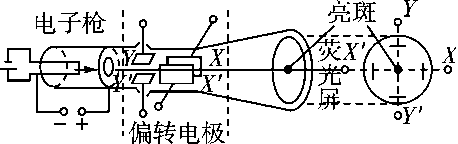
\includegraphics[width=2.08333in,height=0.65625in]{media/image292.png}\end{center}

(2)原理

\ding{172}如果在偏转电极$XX'$和$YY'$之间都没有加电压,则电子枪射出的电子沿直线传播,打在荧光屏\_\_中心\_\_,在那里产生一个亮斑;

\ding{173}$YY'$上加的是待显示的\_\_信号电压\_\_,$XX'$上是机器自身产生的锯齿形电压,叫做扫描电压.若所加扫描电压和信号电压的周期相同,就可以在荧光屏上得到待测信号在一个周期内变化的图象.

\newpage
\subsection{平行板电容器的动态分析}

1.常见类型

\begin{center}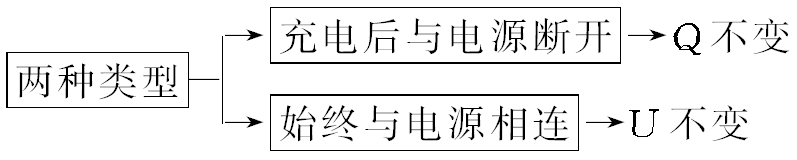
\includegraphics[width=2.51042in,height=0.5in]{media/image295.png}\end{center}

{[}例1{]}(2018·安徽安庆质检)如图所示,先接通开关S使电容器充电,然后断开开关S.当增大两极板间距离时,电容器所带电荷量Q、电容C、两极板间电势差U、电容器两极板间场强E的变化情况是( C )

\begin{center}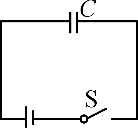
\includegraphics[width=0.625in,height=0.58333in]{media/image296.png}\end{center}

A.Q变小,C不变,U不变,E变小

B.Q变小,C变小,U不变,E不变

C.Q不变,C变小,U变大,E不变

D.Q不变,C变小,U变小,E变小

\begin{solution}
	电容器充电后再断开开关S,其所带的电荷量不变.由$C \alpha \dfrac{\varepsilon_{r} S}{d}$可知,d增大时,C变小时,又因为$U=\dfrac{Q}{C}$,所以U变大,对于场强E,由于$E=\dfrac{U}{d'}$,$U=\dfrac{Q}{C}=\dfrac{Q}{\dfrac{\varepsilon_{r} S}{4 \pi k d}}$,所以$E=\dfrac{U}{d}=\dfrac{4 \pi k d Q}{\varepsilon_{r} S d}=\dfrac{4 \pi k Q}{\varepsilon_{r} S}$.由以上分析可知,间距d增大,E不变.因此选项C正确.
\end{solution}
\begin{center}
\includegraphics[width=0.70833in,height=0.125in]{media/image13.png}

\textbf{解决电容器问题的两个常用技巧}
\end{center}


(1)在电荷量保持不变的情况下,由$E=\dfrac{U}{d}=\dfrac{Q}{Cd} =\dfrac{4 \pi k Q}{\varepsilon_{r} S}$知,电场强度与板间距离无关.

(2)对平行板电容器的有关物理量Q、E、U、C进行讨论时,关键在于弄清哪些是变量,哪些是不变量,在变量中哪些是自变量,哪些是因变量,抓住$C=\dfrac{\varepsilon_{P} S}{4 \pi k d} Q=C U$ 和 $E=\dfrac{U}{d}$进行判定即可.
\newpage
\subsection{带电粒子在电场中的直线运动}

1.带电粒子在电场中运动时是否考虑重力的处理方法

(1)基本粒子:如电子、质子、$\alpha$粒子、离子等,除有说明或明确的暗示以外,一般都不考虑重力(但并不忽略质量).

(2)带电颗粒:如液滴、油滴、尘埃、小球等,除有说明或有明确的暗示以外,一般都要考虑重力.

2.解决带电粒子在电场中的直线运动问题的两种思路

(1)运动状态的分析:带电粒子沿与电场线平行的方向进入匀强电场,受到的电场力与运动方向在同一条直线上,做加(减)速直线运动.

(2)用功与能的观点分析:电场力对带电粒子做的功等于带电粒子动能的变化量,即$q U=\dfrac{1}{2} m v^{2}-\dfrac{1}{2} m v_{0}^2$.

{[}例2{]}一电荷量为q(q\textgreater0)、质量为m的带电粒子在匀强电场的作用下,在t=0时由静止开始运动,电场强度随时间变化的规律如图所示,不计重力,求在t=0到t=T的时间间隔内

(1)粒子位移的大小和方向;

(2)粒子沿初始电场反方向运动的时间.

\begin{center}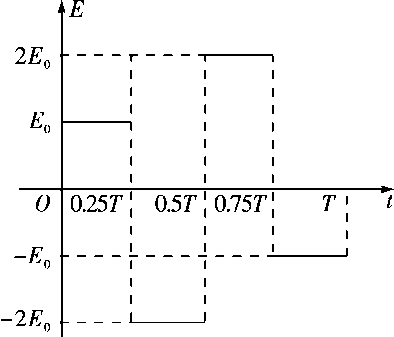
\includegraphics[width=1.79167in,height=1.53125in]{media/image297.png}\end{center}
\begin{solution}
	(1)
	
	(2)
\end{solution}

\begin{center}
\includegraphics[width=0.70833in,height=0.125in]{media/image25.png}

\textbf{带电体在匀强电场中做直线运动的分析思路}
\end{center}


\begin{center}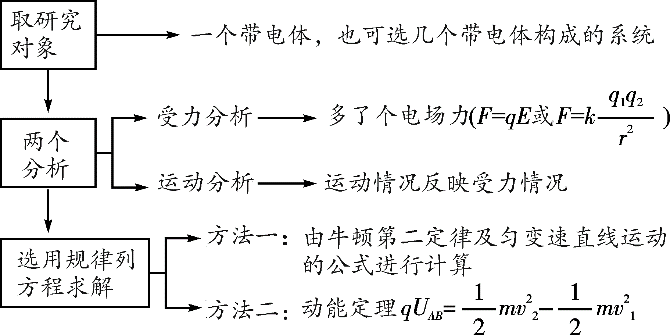
\includegraphics[width=3.04167in,height=1.52083in]{media/image298.png}\end{center}
\newpage
\subsection{带电粒子在电场中的偏转}

1.基本规律:设粒子带电荷量为q,质量为m,两平行金属板间的电压为U,板长为l,板间距离为d(忽略重力影响),则有

\begin{center}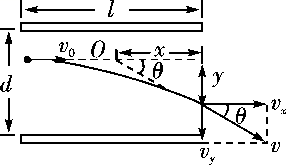
\includegraphics[width=1.30208in,height=0.75in]{media/image299.png}\end{center}

(1)加速度:$a=\dfrac{F}{m}=\dfrac{q E}{m}=\dfrac{q U}{m d}$.

(2)在电场中的运动时间:$t=\dfrac{l}{v_{0}}$.

(3)位移
$\left\{\begin{array}{l}l=v_{x} t=v_{0} t \\ y=\dfrac{1}{2} a t^2\end{array}\right.$

$y=\dfrac{1}{2} a t^{2}=\dfrac{q U R}{2 m v_{0} d}$

(4)速度$\left\{\begin{array}{l}v_{x}=v_{0}, \quad  \\ v_{y}=a t, \quad\end{array}\right.$

$v_{y}=\dfrac{q U t}{m d^{\prime}} \quad v=\sqrt{v_{x}^{2}+v_{y}^{2}}$\quad
$\tan \theta=\dfrac{v_{y}}{v_{x}}=\dfrac{q U l}{m v_{0}^{2} d}$.

2.两个结论

(1)不同的带电粒子从静止开始经过同一电场加速后再从同一偏转电场射出时的偏转角度总是相同的,偏转位移也总是相同的.证明:由$q U_{0}=\dfrac{1}{2} m v_{0}$及$\tan \theta=\dfrac{q U l}{m v_{0} d}$ 得 $\tan \theta=\dfrac{U l}{2 U_{0} d'} ;$ 同理可得 $y=\dfrac{U L^{2}}{4 v_{0} d}$

(2)粒子经电场偏转后,合速度的反向延长线与初速度延长线的交点O为粒子水平位移的中点,即O到电场边缘的距离为$\dfrac{l}{2}$.

3.带电粒子在匀强电场中偏转的功能关系

当讨论带电粒子的末速度v时,也可以从能量的角度进行求解:$q U_{y}=\dfrac{1}{2} m v^{2}-\dfrac{1}{2} m v_{0},$ 其中 $U_{y}=\dfrac{U}{d}y$,指初、末位置间的电势差.

{[}例3{]}如图所示的装置放置在真空中,炽热的金属丝可以发射电子,金属丝和竖直金属板之间加一电压$U_1$=2500V,发射出的电子被加速后,从金属板上的小孔S射出.装置右侧有两个相同的平行金属极板水平正对放置,板长l=6.0cm,相距d=2 cm,两极板间加以电压$U_2$=200V的偏转电场.从小孔S射出的电子恰能沿平行于板面的方向由极板左端中间位置射入偏转电场.已知电子的电荷量$e=1.6\times 10^{-19}C$,电子的质量$m=0.9\times 10^{-30}kg$,设电子离开金属丝时的速度为零,忽略金属极板边缘对电场的影响,不计电子受到的重力.求:

\begin{center}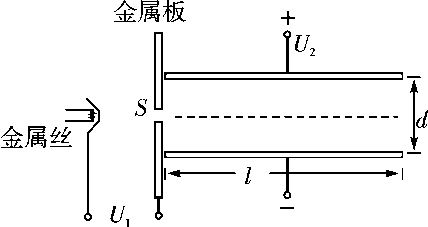
\includegraphics[width=1.94792in,height=1.03125in]{media/image300.png}\end{center}

(1)电子射入偏转电场时的动能$E_k$;

(2)电子射出偏转电场时在竖直方向上的侧移量y;

(3)电子在偏转电场运动的过程中电场力对它所做的功W.

\begin{solution}
	(1)$4.0\times 10^{-16} J$ (2)0.36 cm (3)$5.76\times 10^{-18} J$
\end{solution}
\subsection{带电粒子在交变电场中的运动}

带电粒子在交变电场中运动的分析方法

(1)注重全面分析

分析受力特点和运动规律,抓住粒子的运动具有周期性和空间上具有对称性的特征,求解粒子运动过程中的速度、位移等,并确定与物理过程相关的边界条件.

(2)分析时从两条思路出发

一是力和运动的关系,根据牛顿第二定律及运动学规律分析;二是功能关系,根据动能定理及能量守恒定律分析.

(3)此类题型一般有三种情况

\ding{172}粒子做单向直线运动(一般用牛顿运动定律求解);

\ding{173}粒子做往返运动(一般分段研究);

\ding{174}粒子做偏转运动(一般根据交变电场特点分段研究).

{[}例4{]}(多选)如图甲所示,平行金属板中央有一个静止的电子(不计重力),两板间距离足够大.当两板间加上如图乙所示的交变电压后,在下图中,反映电子速度v、位移x和加速度a三个物理量随时间t的变化规律可能正确的是( AD )

\begin{center}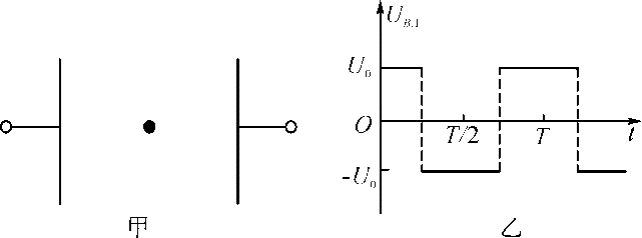
\includegraphics[width=2.91667in,height=1.08333in]{media/image301.png}\end{center}
\begin{center}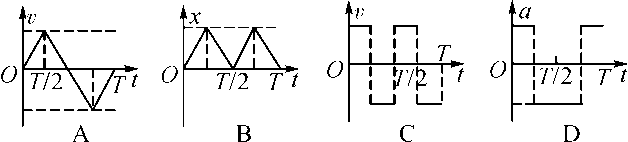
\includegraphics[width=2.85417in,height=0.64583in]{media/image302.png}\end{center}

\begin{solution}
	在平行金属板之间加上如题图乙所示的交变电压时,因为电子在平行金属板间所受的电场力$F=\dfrac{U_{0} e}{d}$,所以电子所受的电场力大小不变.由牛顿第二定律F=ma可知,电子在第一个$\dfrac{T}{4}$内向B板做匀加速直线运动,在第二个$\dfrac{T}{4}$内向B板做匀减速直线运动,在第三个$\dfrac{T}{4}$内反向做匀加速直线运动,在第四个$\dfrac{T}{4}$内向A板做匀减速直线运动,所以a-t图象如图D所示,v-t图象如图A所示;又因匀变速直线运动位移$x=v_0t+\dfrac{1}{2}at^2$,所以x-t图象应是曲线.故选项A、D正确,B、C错误.
\end{solution}
\begin{center}
\includegraphics[width=0.70833in,height=0.125in]{media/image13.png}\end{center}

(1)利用图象

带电粒子在交变电场中运动时,受电场力作用,其加速度、速度等均做周期性变化,借助图象描述它在电场中的运动情况,可直观展示其物理过程,从而快捷地分析求解.

画图象时应注意在v-t图中,加速度相同的运动一定是平行的直线,图象与v-t轴所夹面积表示位移,图象与t轴的交点表示此时速度反向.

(2)利用运动的独立性

对一个复杂的合运动,可以看成是几个分运动合成的.某一方向的分运动不会因其他分运动的存在而受到影响.应用这一原理可以分析带电粒子在交变电场中的运动.根据各分运动的情况,再按运动的合成与分解规律分析合运动情况.
\newpage
\begin{problemset}

\item 概念
	\begin{itemize}
		\item 电场线越密的地方表示电场强度越大
		\item 等势线越密的地方表示电场强度越大;(等差等势线)
		\item 电场线越密(电场强度越大),电势变化越快;
		\item 在匀强电场中,平行线段长度之比等于电势差之比;
		\item 电场方向为电场线方向或电场线切线方向;
		\item 电场线与等势面垂直,并从电势较高的等势面指向电势较低的等势面;
		\item 电势沿电场线方向减小;
		\item 正电荷沿电场线方向移动,做正功,电势减小,电势能减小;
		\item 负电荷沿电场线方向移动,做负功,电势减小,电势能增加。
	\end{itemize}
\item 力场与电场对比
	\begin{itemize}
		\item 重力场\quad 匀强电场
		\begin{longtable}[]{@{}m{2cm}m{4cm}m{3cm}@{}}
		\toprule
		物理量 & 重力场 & 匀强电场\tabularnewline
		\midrule
		\endhead
		力 & $F=ma$ &$F=qE$\tabularnewline
		场强 &$a=\dfrac{F}{m}=g=10m/s^2$ &$E=\dfrac{F}{q}$\tabularnewline
		
		势能&$E_p=mgh$&$E_p=qEd=q\phi$\tabularnewline
		
		势& $gh=\dfrac{E_p}{m}$& $\phi=\dfrac{E_p}{q}$\tabularnewline
		\bottomrule
		\end{longtable}

		\item 引力场\quad 点电荷电场
		\begin{longtable}[]{@{}m{2cm}m{4cm}m{3cm}@{}}
		\toprule
		物理量 & 引力场 & 点电荷电场\tabularnewline
		\midrule
		\endhead
		力 & $F=G\dfrac{Mm}{r^2}$ &$F=k\dfrac{Qq}{r^2}$\tabularnewline
		场强 &$a=\dfrac{F}{m}=G\dfrac{M}{r^2}$ &$E=\dfrac{F}{q}=k\dfrac{Q}{r^2}$\tabularnewline
		
		势能&$E_p=-G\dfrac{Mm}{r}$&$E_p=k\dfrac{Qq}{r}$\tabularnewline
		
		势& $=\dfrac{E_p}{m}=-G\dfrac{M}{r}$& $\phi=\dfrac{E_p}{q}=k\dfrac{Q}{r}$\tabularnewline
		\bottomrule
		\end{longtable}
	\end{itemize}
\end{problemset}

